\chapter{Trainingsdatengenerator}
\label{cha:gui}
Der in dieser Arbeit gewählte Forschungsansatz beinhaltet die Verbesserung des Testens von \gls{gui}-Oberflächen durch Verwendung von Autoencodern. Um diese Autoencoder zu trainieren werden Daten über \gls{gui}-Oberflächen benötigt.

Der erste Schritt, der während der Bearbeitung durchgeführt wurde, ist daher die Entwicklung des Trainingsdatengenerators. Die Trainingsdaten werden hierbei prozedural generiert in Form von validen Ansichten von \glspl{gui}.
Um diesen Generator zu entwickeln wird eine \gls{gui} mit der Programmiersprache Rust als Mock-Applikation nachgebaut. In den nächsten Abschnitten werden daher die Hintergründe der Entscheidung für Rust und die hinter diesem Kapitel stehenden grundlegenden Fragen erläutert.
Darüber hinaus wird ein Framework zur \gls{gui}-Entwicklung benötigt. Im weiteren Verlauf dieses Kapitels werden die Anforderungen an diese Frameworks erklärt, verschiedene Frameworks evaluiert und eines davon zur Entwicklung ausgewählt. Im Anschluss folgt eine Beschreibung und Analyse der Entwicklung des Mocks und des Generators sowie ein Fazit.

Wie in Abschnitt \ref{sec:rust} beschrieben, ist der Grund für den Einsatz von Rust die Ausführungsgeschwindigkeit bei gleichzeitiger Speichersicherheit. Die Ausführungsgeschwindigkeit beeinflusst später die Trainingsgeschwindigkeit. Die Untersuchung der Einsetzbarkeit und der Reife der Sprache Rust und der Frameworks für anschließende Arbeiten ist, wie in Abschnitt \ref{sec:goal} beschrieben, ein sekundäres Ziel dieser Arbeit. Insbesondere ist angedacht, Rust bzw. solche Mocks für das Training der am \gls{fzi} entwickelten Netze zu verwenden. Daher werden in diesem Kapitel nicht nur die für diese Arbeit ausschlaggebenden Anforderungen, sondern darüber hinaus noch Weitere formuliert. Diese werden entsprechend auch zur Analyse und Bewertung der untersuchten Frameworks herangezogen.

Die \gls{gui}, die in dieser Masterarbeit nachgebaut werden soll, ist die des Dekompilierers JADX\footnote{\url{https://github.com/skylot/jadx}, letzter Zugriff: 13.12.2021}, der aus Android DEX\footnote{\url{https://source.android.com/devices/tech/dalvik/dex-format.html}, letzter Zugriff: 13.12.2021}- oder APK\footnote{\url{https://developer.android.com/guide/components/fundamentals}, letzter Zugriff: 13.12.2021}-Dateien Java-Quelltext generiert.
%Ein Screenshot dieser \gls{gui} wird in Abb.~\ref{fig:jadx} dargestellt.
Bei der Implementierung sollen möglichst alle Ansichten von JADX abgedeckt sein. JADX folgt den Betriebssystem-Designsprachen und verwendet viele native Elemente, die je nach Betriebssystem anders aussehen können. Um alle Varianten korrekt abzudecken müssten drei verschiedene Mocks bzw. ein Mock mit drei verschiedenen Designs entwickelt werden. Um diesen Aufwand zu reduzieren, erfolgt in dieser Masterarbeit die Umsetzung des Mocks auf Basis von JADX auf dem Betriebssystem Microsoft Windows 10 Version \mbox{10.0.19043}. Wie sich diese Autoencoder im Bezug auf die Designsprachen anderer Betriebssysteme verhalten, kann in weiteren Arbeiten analysiert werden.


% \begin{figure}
%     \centering
%     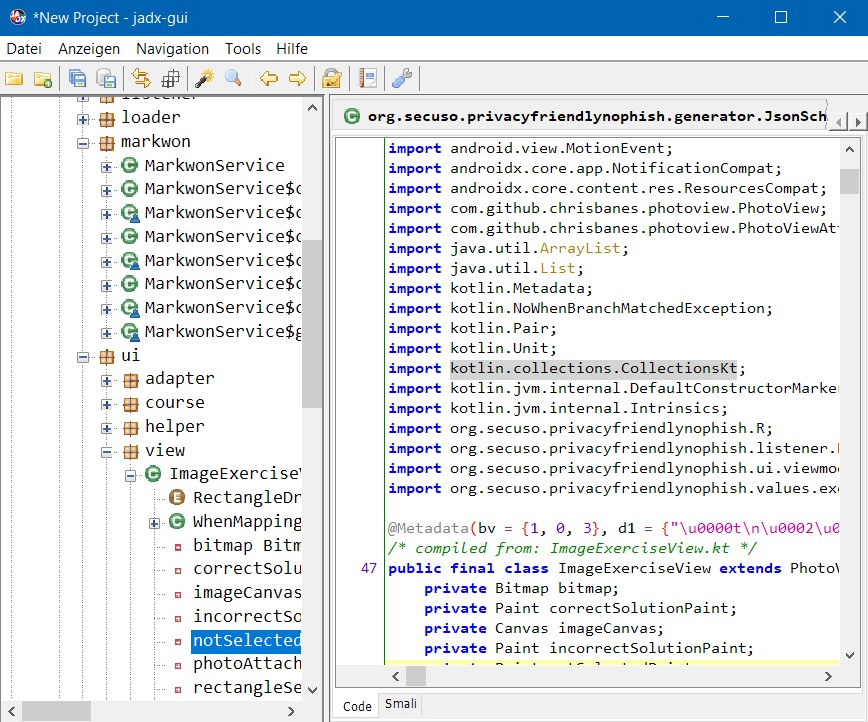
\includegraphics[width=\linewidth]{bilder/jadx.jpg}
%     \caption{GUI-Oberfläche von JADX unter Windows 10} % nicht ins Glossar hinzufügen!
%     \label{fig:jadx}
% \end{figure}


\section{Evaluierung von GUI-Frameworks}
\label{sec:gui-eval}
Nachdem das Vorbild des Mocks und die Gedanken hinter der Untersuchung in diesem Kapitel vorgestellt wurden, werden in diesem Abschnitt Anforderungen an die einzelnen Frameworks formuliert. Anschließend werden diese vorgestellt, dann grob sowie im Detail verglichen. Zum Schluss erfolgt die Auswahl des Frameworks und ein Fazit.

\subsection{Kriterien}
\label{subsec:criteria}
\todo{Aufteilen in Kriterien die gebraucht werden udn welche die erst später gebraucht werden --> Es soll ein Framework eingesetzt werden,
das sich möglichst auch schon für diese Einsatzzwecke eignet}

Eine Anforderung an Frameworks ist, dass diese auf möglichst jeder Desktop-Plattform laufen sollen. Insbesondere muss ein Framework unter Linux lauffähig sein, da der Server, der später den Mock ausführt, Linux verwendet. Darüber hinaus sollen möglichst alle Features in Rust implementiert sein. Einer der Hauptgründe Rust zu verwenden, sind die Vorteile bzgl. der Speichersicherheit. Viele Frameworks sind jedoch beispielsweise in C++ implementiert und werden lediglich über Bindings durch Rust-Applikationen verwendbar gemacht. Solche Frameworks können in Rust in der Regel nur unsicher aufgerufen werden, da C++ keine vergleichbaren Sicherheitsfeatures bietet.

Des Weiteren existieren einige Anforderungen, die nicht für diese Arbeit erfüllt sein müssen, aber in der Zukunft wichtig werden. Dazu gehört die Unterstützung von Offscreen Rendering durch die \gls{gui}-Frameworks. Eine Möglichkeit für Offscreen Rendering soll vorhanden sein, da die einzelnen Ansichten der \gls{gui} zukünftig auf einem Server ohne Verwendung von Betriebssystemfunktionen prozedural generiert werden sollen. Neben der Möglichkeit des Verzichts auf einen Fenstermanager und Betriebssystembibliotheken soll dadurch ein höherer Grad an Parallelisierung ohne Overhead erreicht werden. Bei Offscreen Rendering wird, vereinfacht beschrieben, nicht in ein Betriebssystemfenster (\dh auf den Bildschirm) gerendert. Stattdessen wird \zb im Fall von DirectX ein sog. Render Target~\cite{stevewhimsRenderTargetsOverview} gewählt, das eine Form einer Bitmap darstellt, die sich im Speicher befindet.
Offscreen Rendering ist für das Training der Autoencoder hilfreich. Da als Trainingsdaten lediglich Abbilder benötigt werden, ist es ausreichend, den Buffer (\dh die Bitmap) als Bilddatei abzuspeichern. So können Trainingsdaten ohne den Overhead bei der Initialisierung der Betriebssystem-Fenster generiert werden. Eine unbedingte Notwendigkeit für Offscreen Rendering besteht zum jetzigen Zeitpunkt jedoch nicht. Für die erhoffte Wiederverwendbarkeit im Zuge des Trainings der am \gls{fzi} entwickelten Netze wird Offscreen Rendering jedoch zur Voraussetzung. Hier soll ausschließlich auf der \gls{gpu} gerechnet werden, auf welcher keine Betriebssystemfunktionen zur Verfügung stehen.
Für das reine Generieren von Trainingsdaten ist diese Anforderung nicht notwendig. Die Trainingsdaten im Rahmen dieser Masterarbeit werden vorwiegend auf einem Desktop-PC generiert, auf welchem der Trainingsdatengenerator gestartet wird. Die benötigten Betriebssystemfunktionen stehen somit zur Verfügung.

Eine weitere Anforderung ist, dass das Framework möglichst ausschließlich die \gls{cpu} verwenden und nicht auf der \gls{gpu} rendern soll. Diese Anforderung ist für das reine Training der Autoencoder zunächst von untergeordneter Bedeutung, da hierfür ohne Probleme die \gls{gpu} verwendet werden kann. Da das Training der am \gls{fzi} entwickelten Netze jedoch auf der \gls{gpu} stattfinden soll, könnten Abhängigkeiten zu Grafikschnittstellen, welche zusätzliche \gls{gpu}-Zugriffe verursachen, für Komplikationen sorgen. Daneben ist es sinnvoll, dass die Generierung von Trainingsdaten auch ohne \gls{gpu} funktioniert, beispielsweise wenn diese schon durch andere Prozesse belegt ist. \gls{cpu}-Rendering ist im Vergleich zu Offscreen Rendering von geringerer Bedeutung, da das Nichtvorhandensein den zukünftigen Einsatz des Mocks nicht komplett verhindert, sondern unter Umständen nur die Nutzung der \gls{gpu} komplizierter wird. Des Weiteren könnten hier zukünftig Software-Implementierungen von Grafikschnittstellen wie lavapipe\footnote{\url{https://airlied.blogspot.com/2020/08/vallium-software-swrast-vulkan-layer-faq.html}, letzter Zugriff: 13.12.2021} Abhilfe schaffen. Mit lavapipe ist es möglich, Vulkan-Code ohne eine \gls{gpu} auszuführen. Dieser Ansatz ist jedoch vergleichsweise langsam und in einem frühen Stadium.

Zuletzt sollen die Frameworks möglichst schlank sein und keine Abhängigkeiten zu großen anderen Frameworks wie Qt\footnote{\url{https://www.qt.io/}, letzter Zugriff: 13.12.2021} oder GTK\footnote{\url{https://www.gtk.org/}, letzter Zugriff: 13.12.2021} aufweisen. Zusätzliche Abhängigkeiten erhöhen die Komplexität und verringern die Wahrscheinlichkeit, dass ein Einsatz ohne \gls{gpu}-Zugriffe möglich ist.


\subsection{GUI-Frameworks}

Als Basis für die Evaluierung der Frameworks dienen die Frameworks, die auf der Seite \emph{Are we GUI yet?}~\cite{AreWeGUI} aufgelistet sind. Sogenannte \emph{Are we\dots?}-Seiten werden im Rust-Umfeld traditionell dazu verwendet, den aktuellen Stand der Entwicklung zu einem spezifischen Thema zu darzulegen. Beispiele hierfür geben die Seiten \emph{Are we web yet?}\footnote{\url{https://www.arewewebyet.org}, letzter Zugriff: 13.12.2021} und \emph{Are we game yet?}\footnote{\url{https://arewegameyet.rs/}, letzter Zugriff: 13.12.2021}. Weitere, aktiv entwickelte Frameworks wurden in einer weiterführenden Recherche nicht gefunden. Diese Frameworks der Seite Are we GUI yet? werden in der Tabelle \ref{tab:frameworks} aufgelistet. Bei einigen Einträgen handelt es sich streng genommen um Bibliotheken und damit nicht um Frameworks. Im Unterschied zu Bibliotheken, geben Frameworks anhand von Schnittstellen und abstrakten Implementierungen Richtlinien für die Realisierung einer Lösung vor, welche eine bestimmte Architektur reflektieren~\cite[S.~412]{vogelArchitekturVorgehenWIE2009}. Dahingegen kann der Entwickler bei Verwendung einer Bibliothek selbst entscheiden, wann, wo und wie er diese einsetzt. Da Frameworks jedoch die Mehrheit darstellen und es sich bei den in Frage kommenden Einträgen ausschließlich um Frameworks handelt, wird hier zur besseren Lesbarkeit ausschließlich der Begriff \emph{Framework} verwendet.

In der Tabelle fehlt lediglich der Rust Qt Binding Generator, da dieser Bindings generiert um Rust-Quelltext in Qt aufrufbar zu machen. Damit ist diese Bibliothek nicht zur \gls{gui}-Entwicklung in Rust geeignet und wird daher hier nicht betrachtet. Bezüglich des Stands der Entwicklung der Bibliotheken und Frameworks werden in der Tabelle, soweit möglich, die Angaben des Entwicklers verwendet. Sofern der Entwickler selbst keine Angaben macht, wurden die Einträge als \emph{stabil} klassifiziert, falls die Versionsnummer mindestens 1.0 beträgt und in den anderen Fällen als \emph{instabil} klassifiziert. Azul wurde als \emph{sehr instabil} eingestuft, da hier nur Nightly Builds existieren und damit kein stabilisierter (Alpha- oder Beta-) Release.
Die mittlere Spalte der Tabelle enthält die wichtigsten grundlegenden Werkzeuge, Schnittstellen etc. auf denen das entsprechende Framework basiert. Dazu gehören verwendete Renderer (Raqote, GFX etc.), Grafikschnittstellen (wie OpenGL, Vulkan, DirectX etc.) bzw. deren Wrapper (Glium, wgpu etc.) oder GUI-Frameworks (Qt, GTK etc.). In der Spalte \emph{Anmerkung} befinden sich Anmerkungen zu den GUI-Frameworks sowie besondere Einschränkungen. Die Angabe \emph{Desktop} in der rechten Spalte ist hierbei eine Verallgemeinerung der Plattformen Windows, macOS und Linux/Unix. Diese Bezeichnung wurde gewählt, sofern alle drei Plattformen durch die Entwickler adressiert wurden. Die meisten Frameworks sind nicht in einer stabilen Version vorhanden und die unterstützten Plattformen und Schnittstellen können sich schnell ändern. Als Stichtag für die grobe Evaluierung wurde deshalb der 30.06.2021 gewählt. An diesem Tag musste die Vorauswahl der Frameworks getroffen werden, um genügend Zeit für die Einzelevaluierung und die Erstellung des Trainingsdatengenerators zu haben. Daher sind alle Informationen über Frameworks in diesem Kapitel auf dem Stand dieses Stichtages, um die Entscheidungsgrundlage darzulegen.


\subsection{Vorauswahl}

Die in Tabelle~\ref{tab:frameworks} dargestellten Informationen über die Frameworks lassen eine Vorselektion zu, in der viele Frameworks schon ausgeschlossen werden konnten. Zunächst sind offensichtlicherweise alle Frameworks nicht verwendbar, die den Desktop als Plattform nicht unterstützen. macOS oder Windows reichen hier nicht aus, da der entsprechende Server unter Linux läuft. Demnach entfallen auch eingebettete Plattformen oder das Web als Plattform. Darüber hinaus können auch die beschriebenen, nur in Form von Bindings für Rust bereitstehenden Frameworks aussortiert werden. Frameworks, die Qt oder GTK einsetzen, wurden ebenso aussortiert, da diese kein Offscreen Rendering
%\textcolor{red}{(jedenfalls ist dem Autor nichts bekannt - Quelle?)}
unterstützen, viele Abhängigkeiten haben und sehr groß sind. Nach dieser einfachen Vorselektion bleiben folgende Frameworks übrig: Azul, Conrod, Druid, egui, Iced, KAS und OrbTK.

Azul ist in einem sehr frühen Entwicklungsstadium ohne stabilisierter Release und wurde deshalb im weiteren Verlauf nicht berücksichtigt. Bei der Entwicklung von Druid ist es laut den Entwicklern kein Ziel, in eine benutzerdefinierte Render-Pipeline eingebettet zu werden~\cite{LinebenderDruid2018}. Druid unterstützt Offscreen Rendering aktuell nicht und es ist daher auch unwahrscheinlich, dass dies in Zukunft der Fall sein wird. Zukünftig wird genau dies jedoch benötigt, weshalb Druid ebenso nicht weiter berücksichtigt wurde.

Von den verbleibenden Frameworks verwendet ausschließlich OrbTK \gls{cpu}-Rendering mit der Bibliothek \emph{raqote}\footnote{\url{https://github.com/jrmuizel/raqote}, letzter Zugriff: 13.12.2021}. Die Frameworks Iced und KAS verwenden wgpu\footnote{\url{https://wgpu.rs/}, letzter Zugriff: 13.12.2021}, das eine Abstraktionsschicht für native Grafikschnittstellen wie Vulkan, Metal oder DirectX darstellt. Conrod oder egui bieten mehrere Backends an. Bei diesen kann es sich um Wrapper für Grafikschnittstellen, etwa in Form von Glium\footnote{\url{https://github.com/glium/glium}, letzter Zugriff: 13.12.2021} für OpenGL oder Vulkano\footnote{\url{https://github.com/vulkano-rs/vulkano}, letzter Zugriff: 13.12.2021} für Vulkan, oder um Grafik-Engines, \gls{gpu}-Rendering-Bibliotheken etc. handeln. Wie in Abschnitt~\ref{subsec:criteria} beschrieben wurde, ist \gls{cpu}-Rendering keine Anforderung, die auf jeden Fall erfüllt sein muss, da verschiedene Maßnahmen denkbar sind um das dort beschriebene Problem zu umgehen. \gls{gpu}-Rendering-Frameworks wurden daher vorerst weiter mit einbezogen.

\renewcommand{\tabularxcolumn}[1]{>{\raggedright\arraybackslash}p{#1}}
\newcolumntype{s}{>{\hsize=.84\hsize}X}
% \newcolumntype{l}{>{\hsize=.8\hsize}X}

% \begin{table}[htbp!]
%     \begin{center}
%         \caption{Klassifikationsergebnisse Kategorie \glqq Eingabedaten\grqq}
%         \bigskip

        \pgfplotstabletypeset[
            reset styles,
            debug=true,
            string type,
            header=false,
            col sep=semicolon,
            row sep=newline,
            column type=,
            skip first n=1,
            begin table={
              \begingroup\renewcommand{\arraystretch}{1.5}
              \begin{xltabular}{\textwidth}{XXXXXX}
                \caption{Untersuchte GUI-Bibliotheken und -Frameworks (Stand: 30.06.2021)} \label{tab:frameworks} \\
              \toprule
              \textbf{Name} & \textbf{Stand} & \textbf{Renderer / basiert auf / Schnittstelle} & \textbf{Anmerkung} & \textbf{Plattform} \\
              \midrule
              \endhead
            },
            end table={\bottomrule \end{xltabular}\endgroup},
            every head row/.style={ output empty row },  % suppress printing head row (numbers)
            % every head row/.style={after row=\midrule},
            % display columns/0/.style={string type,column name={\textbf{Name}}
            % },
            % display columns/1/.style={string type,column name={\textbf{Stand}}},
            % display columns/2/.style={string type,column name={\textbf{Renderer / basiert auf / Schnittstelle}}},
            % display columns/3/.style={string type,column name={\textbf{Anmerkung}}},
            % display columns/4/.style={string type,column name={\textbf{Plattform}}},
          ]{tabellen/FrameworksTabelle.csv}
%         \label{table1}
%     \end{center}
% \end{table}



\subsection{Detailvergleich}

Die verbleibenden Frameworks wurden detaillierter untersucht und gegebenenfalls Tests unterzogen. %Hier ist es nicht mehr möglich, eine Entscheidung ausschließlich anhand harter Kriterien zu treffen.
Die in Abschnitt \ref{sec:gui-eval} beschriebenen Kriterien werden von allen Frameworks außer OrbTK gleichermaßen erfüllt bzw. im Fall des \gls{cpu}-Renderings nicht erfüllt.
Weitere Entscheidungskriterien sind nun beispielsweise die Qualität der Dokumentation, die Entwicklungsaktivität, Kommunikationsmöglichkeiten mit den Entwicklern sowie die Unterstützung oder Verwendung möglichst etablierter Bibliotheken und Schnittstellen. Gute Kommunikationsmöglichkeiten mit den Entwicklern sind in diesem Fall besonders wichtig, da sich viele Frameworks noch in einem frühen Stadium befinden, in welchem die Dokumentation oft nur unvollständig vorhanden ist. Des Weiteren ist Offscreen Rendering kein zentrales Feature der meisten Frameworks und daher in der Regel nicht oder nur schlecht dokumentiert. Eine Übersicht der Entscheidungsgrundlage wird in Tabelle~\ref{table:frameworks_detail} dargestellt.


\begin{table}[htbp]
    \begin{center}

\rotatebox{90}{%
  \begin{minipage}{.85\textheight}
    \captionof{table}{Bewertung von GUI-Frameworks anhand weicher Kriterien}
    \label{table:frameworks_detail}
        \renewcommand{\arraystretch}{1.5}

        \begin{tabularx}{\textwidth}{ XXXXX }
            \toprule
            OrbTK & Iced  & KAS   & egui & Conrod \\
            \hline
            ++ \gls{cpu}-Rendering & + wgpu-Unterstützung & + wgpu-Unterstützung & + viele unterstützte Grafik-Backends, wgpu nur über 3rd-Party & + viele unterstützte Grafik-Backends \\
            + Entwicklerchat & + größte Entwicklergemeinschaft & + starke Entwicklertätigkeit & + starke Entwicklertätigkeit und mehrere Entwickler     & + starke Entwicklertätigkeit \\
            + Dokumentation durch Readmes, Chat, Beispiele und Rust Docs & + Entwicklerchat & - nur ein Hauptentwickler & + Diskussionsräume & o Anfänge eines Handbuchs, sonst nur Rust Docs \\
            - Geringer Entwicklungsfortschritt & + Dokumentation durch Readmes, Chat, Beispiele und Rust Docs & - Wenig Dokumentation abseits Beispiele & + Dokumentation durch Get Started, Diskussionen und Rust Docs & - Keine Beispiele \\
            - Nur ein Hauptentwickler & - etwas weniger Entwicklung in letzter Zeit & - leere Diskussionsräume & o Immediate Mode Toolkit & - kein Chat / Forum \\

            \bottomrule
        \end{tabularx}

\end{minipage}
}
\end{center}
\end{table}

\subsubsection*{Frameworks mit \gls{gpu}-Rendering}

Vor einer Beschreibung der einzelnen Frameworks ist es wichtig, die Bibliothek \mbox{wgpu} vorzustellen, welche in mehreren Frameworks verwendet wird. wgpu~\cite{GfxrsWgpu2018} ist eine Rust-native WebGPU\footnote{\url{https://www.w3.org/TR/webgpu/}, letzter Zugriff: 13.12.2021}-Implementierung, welche sich durch eine aktive Community auszeichnet. Die Entwicklung wird als Bestandteil von Firefox~\cite{GpuwebGpuwebImplementation2017} u.\,a. durch Mitarbeiter von Mozilla getragen~\cite{GfxrsWgpuPulse2018}, wobei WebGPU als Standard voraussichtlich durch das World Wide Web Consortium\footnote{\url{https://www.w3.org/}, letzter Zugriff: 13.12.2021} anerkannt wird~\cite{WebGPU}. Darüber hinaus unterstützt wgpu mehrere Grafikschnittstellen. Durch eine größere Anzahl an unterstützten Schnittstellen ist es wahrscheinlicher, dass für eine Schnittstelle eine reine Software-Implementierung existiert, welche eingesetzt werden kann. Ein Beispiel dafür ist lavapipe für Vulkan, wie in Abschnitt~\ref{subsec:criteria} beschrieben wurde.

\textbf{Iced~\cite{ramonHecrjIced2019}} ist ein \gls{gui}-Framework, das durch die \gls{gui}-Beschreibungssprache Elm\footnote{\url{https://elm-lang.org/}, letzter Zugriff: 13.12.2021} inspiriert ist. Iced legt laut eigenen Angaben einen Fokus auf Einfachheit und Typsicherheit und basiert auf der Bibliothek wgpu. Es existiert mit 12.100 Sternen auf Github, Commits von 89 verschiedenen Autoren \cite{ramonHecrjIced2019} und einem sehr aktiven Entwicklerchat \cite{IcedZulip} eine vergleichsweise große Entwicklergemeinschaft. Über den Chat können Fragen zur Nutzung geklärt werden, Diskussionen über die Weiterentwicklung stattfinden und Bugreports eingestellt werden.

\textbf{KAS~\cite{KasguiKas2019}} hat gegenüber Iced mit nur zwei Autoren eine deutlich kleinere Entwicklergemeinschaft und wesentlich weniger Dokumentation.
Das Framework ist durch Qt\footnote{\url{https://www.qt.io/}, letzter Zugriff: 13.12.2021} inspiriert und fokussiert sich nach eigenen Angaben auf Typsicherheit und eine schnelle, effiziente und responsive Benutzerschnittstelle. KAS unterstützt ebenfalls wgpu.

\textbf{egui~\cite{ernerfeldtEmilkEgui2019}} wird von den Autoren als Immediate Mode Toolkit bezeichnet, welche laut eigener Aussage die Eigenschaft haben, besonders einfach und unkompliziert zu sein, jedoch nur eingeschränkte Layout-Möglichkeiten bieten. egui zielt darauf ab, die am einfachsten zu benutzende \gls{gui}-Bibliothek zu sein und unterstützt eine große Anzahl an Integrationen (Web, Glium\footnote{\label{footn:glium}\url{https://github.com/glium/glium}, letzter Zugriff: 13.12.2021}, Bevy Game Engine\footnote{\url{https://bevyengine.org/}, letzter Zugriff: 13.12.2021}, Vulkano\footnote{\label{footn:vulkano}\url{https://github.com/vulkano-rs/vulkano}, letzter Zugriff: 13.12.2021},\dots). Vor dem Hintergrund, dass auch komplexere GUIs durch den Mock dargestellt werden sollen, könnte diese Eigenschaft in Zukunft zu Limitierungen führen.

\textbf{Conrod~\cite{PistonDevelopersConrod2014}} kombiniert laut eigener Aussage die Vorteile von Immediate Mode Toolkits mit denen klassischer \gls{gui}-Frameworks. Es bietet Unterstützung für GFX\footnote{\url{https://github.com/gfx-rs/gfx}, letzter Zugriff: 13.12.2021}, Glium\footnoteref{footn:glium}, OpenGl und Vulkano\footnoteref{footn:vulkano}. Conrod ist sehr unvollständig dokumentiert, da außer einer kurzen Anleitung, bei dem die meisten Kapitel noch nicht umgesetzt wurden, und Rust Docs keine Dokumentation existiert. Darüber hinaus existiert bei Conrod keine schnelle Kommunikationsmöglichkeit mit den Entwicklern oder anderen Nutzern.

\todo{Vor Abgabe: Angaben zu Frameworks checken! (insbesondere unterstützte Schnittstellen, etc.)}

\subsubsection*{Framework mit CPU-Rendering}
%\todo{Viel von dieser Info in nächstes Kapitel schieben}
\textbf{OrbTK} ist ein Framework, das zum Ziel hat, skalierbare Benutzerschnittstellen zu ermöglichen. Es basiert auf dem Entity-Component-System-Entwurfsmuster, welches aus der Videospielentwicklung stammt~\cite{muratetAccessibilitySeriousGames2020}, und verwendet Elemente des funktionalen sowie des reaktiven Programmierens \cite{RedoxosOrbtk2015}. Das Framework bietet den Vorteil, dass nur auf der \gls{cpu} gerendert wird und daher keine Abhängigkeiten zur Hardware bestehen. Eigene Tests mit OrbTK und Rücksprachen mit dem Entwickler~\cite{blasiusMomentItIt,blasiusHiDifficultSay} brachten das Ergebnis hervor, dass es zum aktuellen Zeitpunkt jedoch nicht möglich ist in einen Framebuffer ohne die Erstellung eines Fensters durch das Betriebssystem zu rendern. Aktuell würde jedoch der Quelltext überarbeitet und einige Komponenten entkoppelt, sodass dies in Zukunft möglich sei. Der gesteckte Zeitrahmen von mehreren Wochen bis Monaten ist dabei für eine produktive Verwendung im Rahmen dieser Masterarbeit zu lang. Dieser lange Zeitraum kommt durch die im Juli/August 2021 eher langsam verlaufende Entwicklung zustande~\cite{blasiusHiDifficultSay}. Zu diesem Zeitpunkt trug nur ein Entwickler in größerem Maß zum Projekt bei. Wie in Abschnitt~\ref{sec:gui-eval} beschrieben, ist Offscreen Rendering jedoch nicht allein ausschlaggebend für oder gegen eine Verwendung eines Frameworks, da die Trainingsdaten auch ohne dieses Feature generiert werden können.

Die Einarbeitungszeit bei OrbTK war kurz. Widgets, die Blöcke, aus denen eine \gls{gui} gebaut wird, können einfach komponiert und per Builder-Entwurfsmuster konfiguriert werden~\cite{RedoxosOrbtk2015}. Die Arbeit mit OrbTK war zu Beginn durch eine sehr schlechte Performance im Vergleich zu anderen Frameworks geprägt. Bereits bei einfachen Anwendungen kam es zu um mehrere Sekunden verzögerte Reaktionen auf Eingaben durch den Benutzer. Dieses Problem konnte jedoch dadurch behoben werden, dass das Release-Profil von Rust ausgewählt wurde. Bei diesem Profil verzichtet Rust auf viele Überprüfungen und führt Optimierungen durch~\cite{CustomizingBuildsRelease}. Eine Erklärungsmöglichkeit hierfür ist, dass bei OrbTK auch das Rendering durch Rust-Bibliotheken durchgeführt wird und nicht durch Grafikschnittstellen übernommen wird. Dadurch wird der Quelltext, welcher das Rendering durchführt, im Gegensatz zu anderen Frameworks erst durch das Release-Profil optimiert und ist nicht bereits voroptimiert. Overlays und zusätzliche Fenster sind mit OrbTK einfach umzusetzen.

\subsubsection*{Entscheidung}

Unter den Frameworks, die eine \gls{gpu} benötigen, ist Iced das vielversprechendste. Erste Tests mit Iced, in welchen das Menü und die Werkzeugleiste von JADX nachgebaut wurden, bestätigten dies. Die Einarbeitungszeit war verhältnismäßig gering und alle verbleibenden offenen Fragen konnten schnell im Entwicklerchat geklärt werden. Das Layout-System sowie die Erstellung von Komponenten funktionierte zuverlässig.

Bestimmte Funktionalitäten wie Overlays oder zusätzliche Betriebssystemfenster sind zum aktuellen Zeitpunkt nur unvollständig bzw. nicht umgesetzt.
Eine weitere Limitierung ist, dass Iced zunächst eine \gls{gpu} benötigt. Die verwendete Bibliothek wgpu setzt auf Vulkan und Metal -- eine Umsetzung für DirectX ist geplant~\cite{GfxrsWgpu2018}. Die am weitesten verbreiteten Implementierungen dieser Grafikschnittstellen benötigen zwar eine \gls{gpu}, eine rein \gls{cpu}-basierte Implementierung ist jedoch denkbar.

OrbTK ist durch das \gls{cpu}-Rendering in Zukunft unkompliziert durch das FZI zu verwenden. Da außerdem Features wie zusätzliche Fenster und Overlays existieren und trotz der recht kleinen Entwicklergemeinschaft fiel die Entscheidung auf OrbTK.





\section{Implementierung des Mocks}
\label{sec:impl}
Der Mock wurde unter Einsatz des Frameworks \emph{OrbTK} implementiert. Da die prozedurale Generierung, und damit die Variabilität, erst in späteren Schritten entwickelt wird, wurde in diesem Schritt JADX mit so wenigen Veränderungen wie möglich abgebildet. In diesem Abschnitt sollen das Ziel des Mocks und die Vor- und Nachteile der Entwicklung mit OrbTK erläutert werden, bevor die Eigenschaften und Limitierungen der Implementierung beschrieben werden.

\subsection{Ziel des Mocks}
\label{subsec:goal_mock}
Das Ziel hinter der Entwicklung dieses Mocks ist es, eine Datenquelle zu schaffen, die zum Training von Autoencodern verwendet werden kann. Diese Datenquelle soll aus validen Abbildern von \gls{gui}-Oberflächen bestehen und sich an der Anwendung JADX orientieren. Dabei geht es vorwiegend darum, real aussehende \glspl{gui} zu erstellen um herauszufinden, ob und wie \gls{gui}-Oberflächen von Autoencodern enkodiert werden können. Eine exakte Nachbildung von JADX ist daher nicht nötig und aus Gründen des Zeitaufwandes auch nicht sinnvoll. Es wird allein deshalb zu Abweichungen kommen, da OrbTK sich nicht an der Windows-Designsprache oder dem Design von JADX orientiert.

Eine sekundär zu beantwortende Frage ist, wie gut die Autoencoder noch mit der realen \gls{gui} von JADX funktionieren. In Kapitel \ref{cha:autoencoder} wird daher untersucht, inwiefern die Abweichungen zwischen Mock und realer \gls{gui} einen Effekt auf die Ergebnisse der Autoencoder haben.

Die Implementierung dieses Mocks wird in dieser Arbeit außerdem so beschränkt, dass nur \gls{gui}-Elemente, die Teil von JADX sind, umgesetzt werden. Funktionen, die durch das Betriebssystem bereitgestellt werden, sind ausgenommen. Hiervon sind Dialoge zum Öffnen von Dateien sowie zur Auswahl von Schriftarten betroffen.

\subsection{OrbTK}
Mit OrbTK war es möglich, alle wichtigen \gls{gui}-Elemente in zufriedenstellender Qualität umzusetzen. Das Framework setzt auf Widgets, die den Kern darstellen und jeweils einem \gls{gui}-Element entsprechen. Widgets können komponiert werden, um neue Widgets zu kreieren. Das Aussehen kann über das Setzen von Parametern per Builder-Entwurfsmuster verändert werden, das OrbTK umsetzt \cite{RedoxosOrbtk2015}. Alternativ können Theme-Dateien verändert werden, in denen Stile definiert werden können, die während des Startens der Applikation geladen werden. Für die Entwicklung im Rahmen dieser Masterarbeit wurden die Widgets in Komponenten und Elemente aufgeteilt. Komponenten stellen größere Bausteine dar, die eine eigene Funktion darstellen oder mindestens aus mehreren Elementen zusammengesetzt sind. Elemente sind grundlegende Bausteine der \gls{gui}, wie Buttons, Eingabefelder oder Beschriftungen.

Der größte Nachteil von OrbTK ist das Layout-System, das nicht immer fehlerfrei arbeitet. Während der Implementierung kam es häufiger vor, dass \gls{gui}-Elemente ihre Position verändern, ohne, dass der Grund für diese Veränderung ersichtlich war. Darüber hinaus kann es vorkommen, dass das Setzen von Parametern keinen Effekt hat. Beispielsweise haben die Parameter, um die Höhe und Breite von \gls{gui}-Elementen zu setzen, teilweise keine Funktion, wenn sich ein Element innerhalb eines Eltern-Elements befindet. Dieses Verhalten trat scheinbar zufällig auf und war nicht reproduzierbar.

% Kind-Elemente scheinen sich oft ihrem Eltern-Element in der Größe anzupassen. In diesen Fällen sind die einzigen Möglichkeiten, die Größe von Kind-Elementen anzupassen, Grid-Layouts und Margins, welche jedoch wieder Probleme hinsichtlich responsivem Verhalten mit sich bringen und nur beschränkt konfigurierbar sind. Die Komplexität des Layouts ist insgesamt nicht mit der Komplexität der Stylesheet-Sprache CSS vergleichbar.

Außerdem ist es nicht möglich Parameter, die in speziellen Theme-Dateien gespeichert sind, im Anschluss programmatisch zu überschreiben. Theme-Dateien bieten die Möglichkeit, wiederverwendbare Stile für einzelne \gls{gui}-Elemente zu definieren. Wenn solche Parameter einmal gesetzt wurden, können sie im Rust-Quelltext nicht mehr überschrieben werden. Der in Rust gesetzte Parameter wird ignoriert. Neben dem fehlenden Fehlerfeedback ist das problematisch, da so ein neuer Style in der Theme-Datei für ein einzelnes \gls{gui}-Element definiert werden muss und die Theme-Datei dadurch unnötig fragmentiert. Eine andere Möglichkeit ist, die Parameter im Rust-Quelltext und nicht mehr in der Theme-Datei zu setzen. Dieses Vorgehen führt jedoch zu dupliziertem Quelltext.

Bei OrbTK ist es des Weiteren schwer, Fehler zu identifizieren, da bestimmte Parameter nicht typsicher sind. Die horizontale und vertikale Ausrichtung von Elementen oder das Layout von Grids werden beispielsweise nur als String angegeben. Die Höhe und Breite von Elementen wird als Gleitkommazahl erwartet. Wird stattdessen eine Ganzzahl übergeben, ignoriert OrbTK diesen Wert und gibt keine Fehlermeldung aus. Wenn solche Probleme auftreten und das Aussehen der \gls{gui} nicht mit dem gewünschten Layout übereinstimmt, gibt es kaum Möglichkeiten zu debuggen. Rust-Debugger helfen hier oft nicht weiter, da das entsprechende Verhalten sehr tief in OrbTK auftritt und nicht im Quelltext des Benutzers. Da zusätzlich meist keine Dokumentation vorhanden ist, war so nur \emph{Trial and Error} als Lösungsstrategie möglich.

\subsection{Eigenschaften}

Um JADX abzubilden, wurden die wichtigsten Ansichten von JADX im Mock nachgebaut. Hierzu zählen die Hauptansicht, die Ansicht für die Einstellungen, die Ansichten für Text- und Klassensuche und die Ansicht für die Suche nach Benutzung von Java-Klassen, Attributen und Parametern. Daneben existieren Ansichten für Lognachrichten, das Umbenennen von einzelnen Paketen und Java-Entitäten sowie die About-Ansicht. Alle Ansichten werden entsprechend in neuen Fenstern geöffnet und sind, bis auf die Ansicht für Lognachrichten, im Mock vorhanden. Einige davon werden in den Abb. \ref{fig:mock_comparison} bis \ref{fig:mock_search_comparison} gegenübergestellt.

Ein besonderer Fokus lag darauf, Gruppierungen von \gls{gui}-Elementen möglichst detailgetreu abzubilden. Container, die solche Elemente beinhalten, und Abgrenzungen, welche diese separieren, wurden entsprechend nachgebaut. Die Buttons, Menüs, Eingabefelder etc. wurden entsprechend in ihrem Aussehen angeglichen und, wenn nicht verfügbar, nachgebaut. Um Buttons und \gls{gui}-Elemente zu erstellen wurden die in JADX eingebetteten Bilder und Icons wiederverwendet.

% Während der Entwicklung wurden in diesem Schritt auch schon Logiken umgesetzt, um Daten zur Laufzeit hinzuzufügen und zu verändern. Die \gls{gui} wurde somit nicht hart kodiert. Durch diese Maßnahmen kann ein Generator, der gültige Instanzen der \gls{gui} zufällig erzeugen soll, leichter geschrieben werden. Des Weiteren wurde auf eine möglichst responsive Umsetzung geachtet, um die Umsetzung der prozeduralen Generierung zu vereinfachen.


\begin{figure}[p]
    \centering
    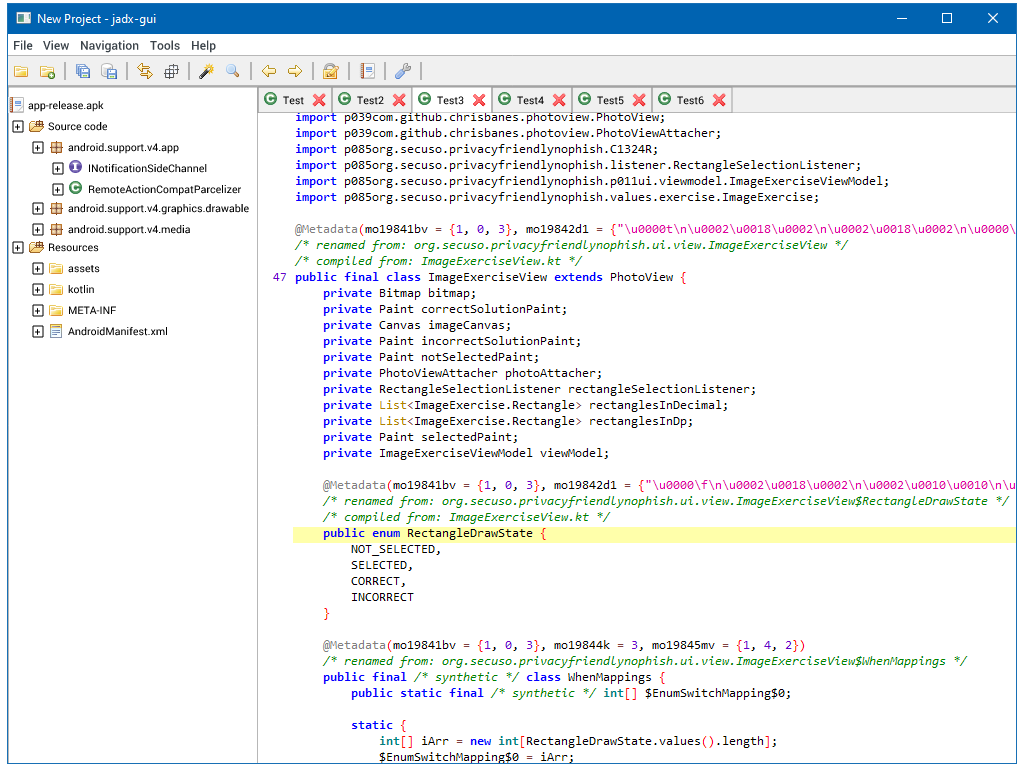
\includegraphics[height=.45\textheight]{bilder/jadx_mock_main.png}
    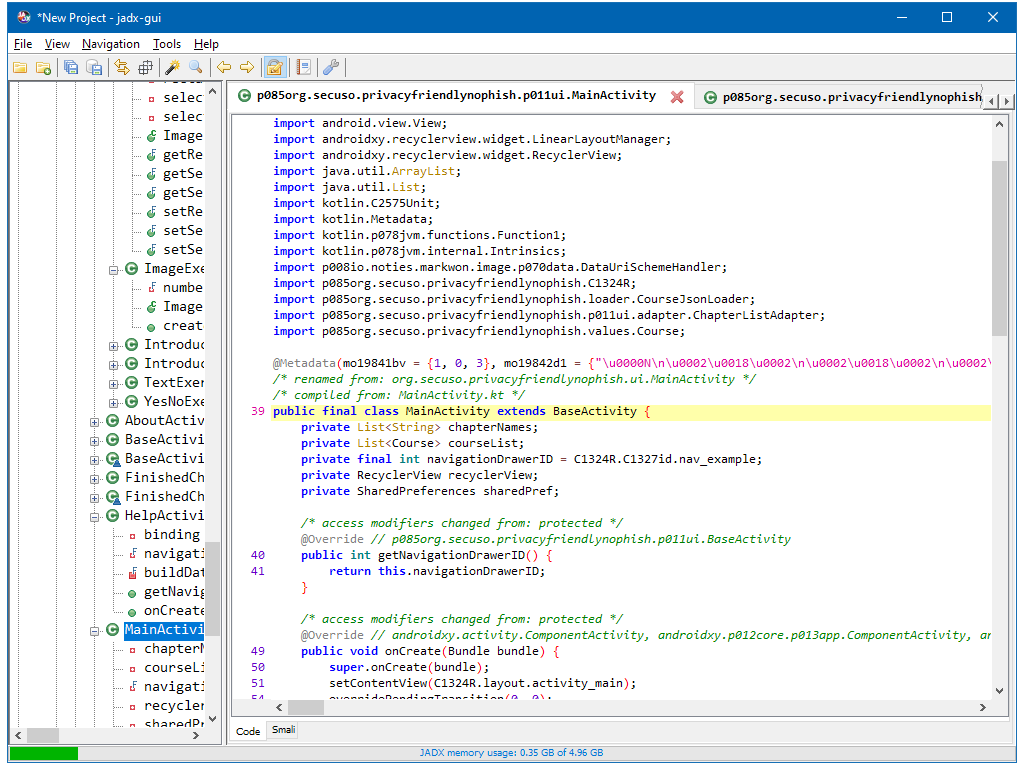
\includegraphics[height=.45\textheight]{bilder/jadx_main.png}
    \caption{Vergleich Hauptansicht: Mock (oben) und JADX (unten)}
    \label{fig:mock_comparison}
\end{figure}

\begin{figure}[p]
    \centering
    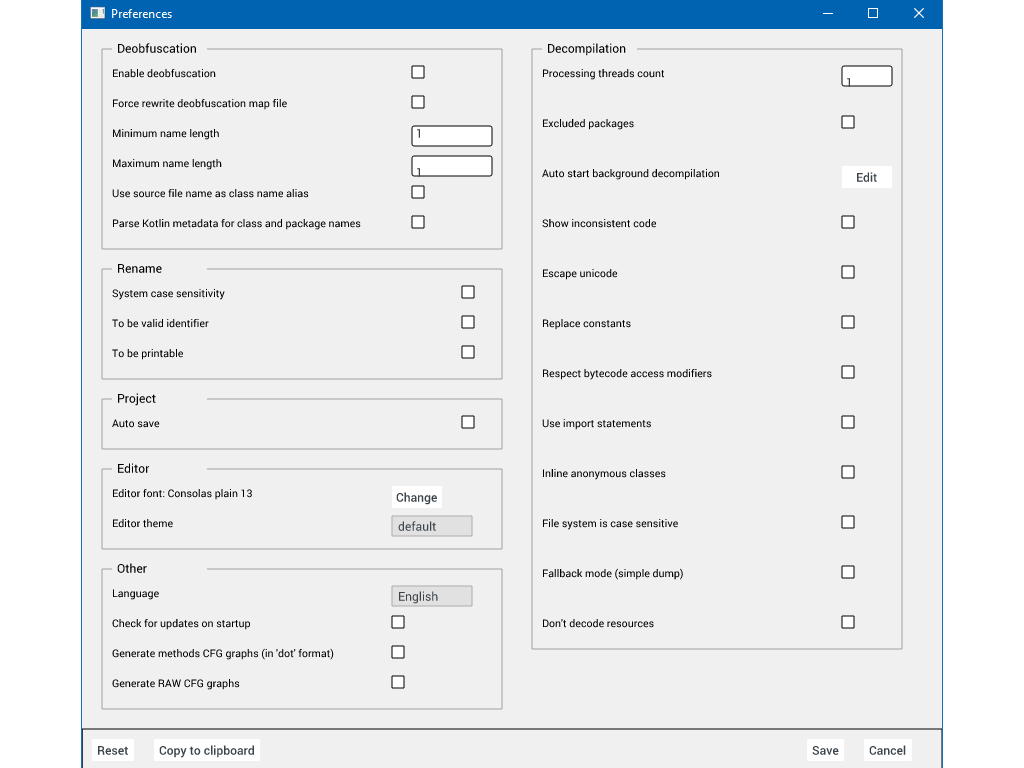
\includegraphics[height=.45\textheight]{bilder/jadx_mock_settings.png}
    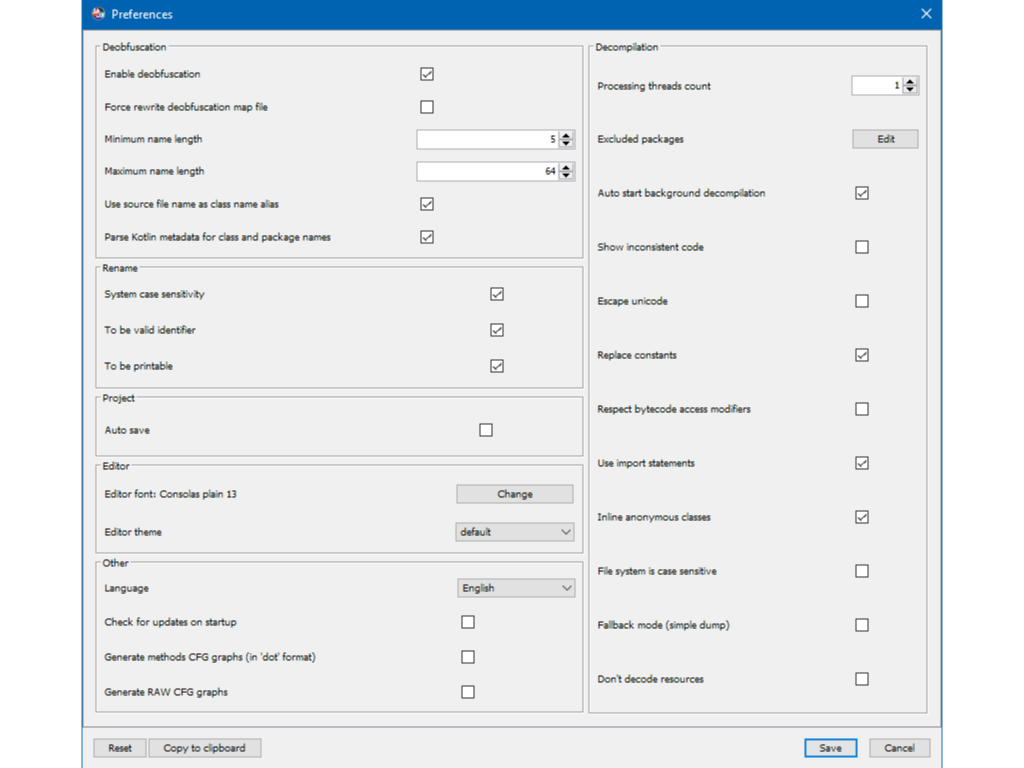
\includegraphics[height=.45\textheight]{bilder/jadx_settings.png}
    \caption{Vergleich Einstellungen: Mock (oben) und JADX (unten)}
    \label{fig:mock_settings_comparison}
\end{figure}

\begin{figure}[p]
    \centering
    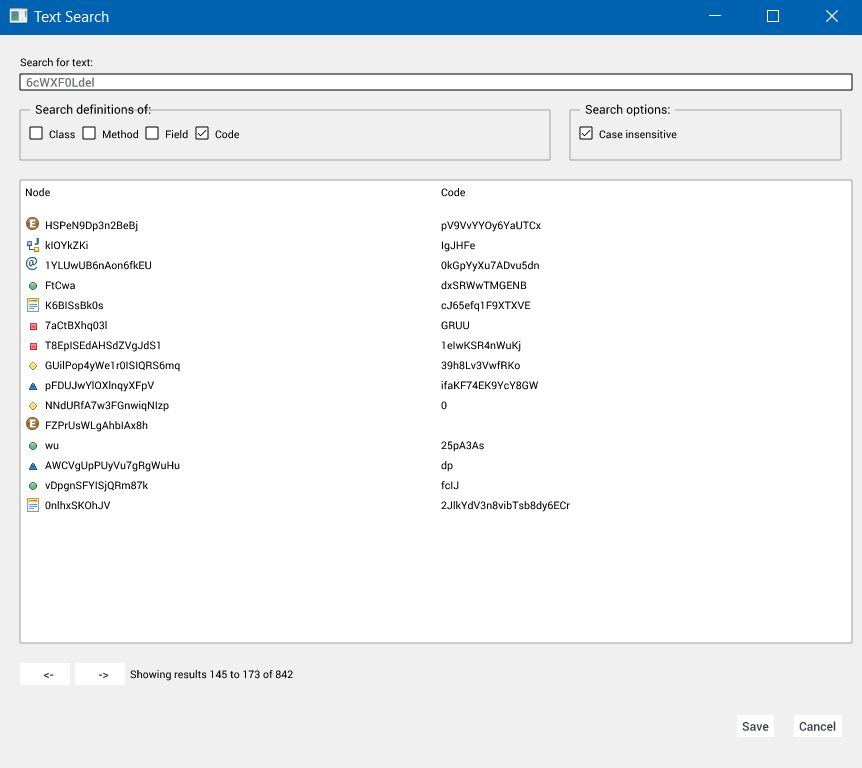
\includegraphics[height=.45\textheight]{bilder/jadx_mock_search.png}
    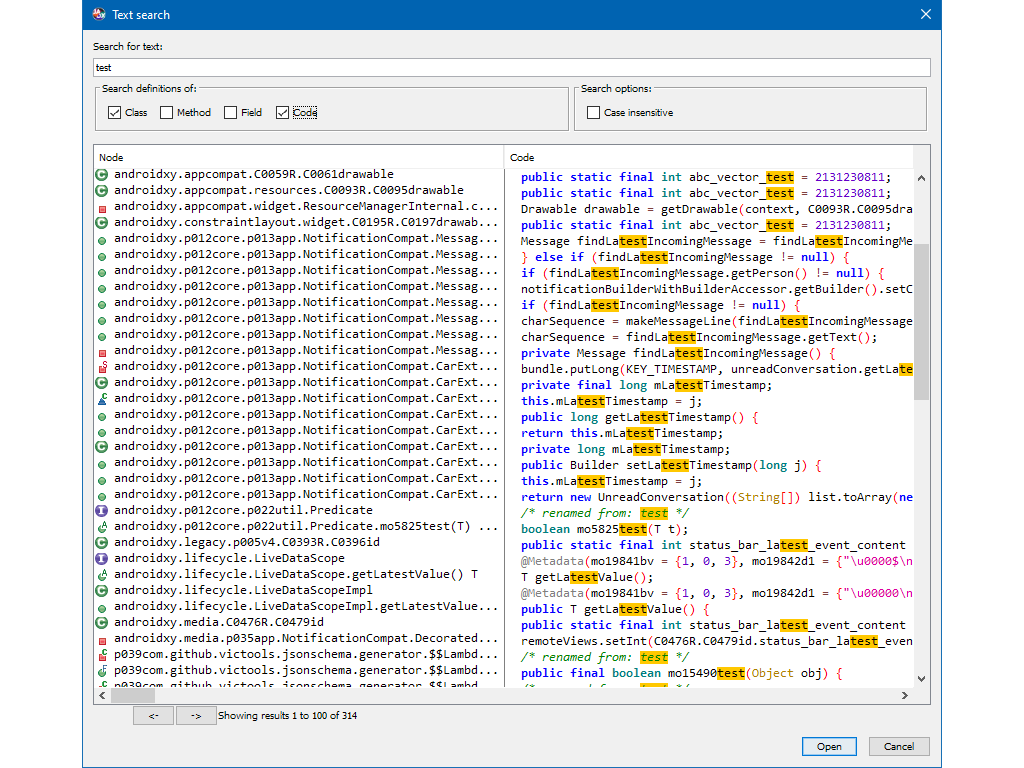
\includegraphics[height=.45\textheight]{bilder/jadx_search.png}
    \caption{Vergleich Text- / Klassensuche: Mock (oben) und JADX (unten)}
    \label{fig:mock_search_comparison}
\end{figure}





\subsection{Limitierungen}
\label{sec:mock_limitations}



Die Limitierungen der Umsetzung ergeben sich zunächst aus den Limitierungen und Fehlern von OrbTK, insbesondere der Rendering-Funktionen. Die meisten Elemente aus JADX sind nicht in OrbTK vorhanden, weshalb sie nachgebaut werden mussten. Das Design der JADX-Applikation, das sich an Windows-Designsprachen orientiert, konnte nicht immer exakt umgesetzt werden, sodass sich kleinere Abweichungen ergeben. OrbTK bietet die Möglichkeit Rahmen um Container innerhalb der Applikation zu ziehen, ähnlich wie sie in JADX oft verwendet werden. Selbst ein Rahmen der Breite \texttt{1}, die kleinste darstellbare Breite, erscheint dicker, als die innerhalb JADX verwendeten Rahmen. Weitere Features wie Schattierungseffekte oder gepunktete Linien (beispielsweise Verbindungslinien des Projekt-Baums in der Hauptansicht von JADX) sind nicht in OrbTK verfügbar.

\todo{Sind diese Abweichungein ein Problem? --> Später in der Arbeit genauer erörtern und Testset aus richtiger JADX-Applikation verwenden}

Die Funktionalität, um mehrere Fenster zu öffnen, ist in OrbTK grundsätzlich vorhanden. JADX verwendet dies beispielsweise um eine Volltext- oder Klassensuche durchzuführen. Das Öffnen zusätzlicher Fenstern ist in OrbTK jedoch aktuell noch sehr fehlerhaft. Wenn die Fenstergröße nach dem Öffnen beispielsweise durch den Mauszeiger verändert wird, wird der Inhalt des Fensters schwarz. Für diese Masterarbeit ist dieser Umstand jedoch kein Problem, da Fenster nur einmal gerendert werden, bevor sie als Bild gespeichert werden. Dadurch finden nach dem initialen Rendering keine Veränderungen mehr statt. Es existieren ähnliche Probleme bezüglich der Ausführung von Aktionen durch den Benutzer. In zusätzlichen Fenstern werden Mausklicks oft nicht registriert, sodass diese mehrfach durchgeführt werden müssen. Auch diese Fehler sind für diesen Anwendungsfall nicht relevant, da für die Experimente im Rahmen dieser Arbeit keine Aktionen mit der Maus durchgeführt werden. Alle Felder, die innerhalb von JADX erreichbar sind, werden vorausgefüllt.

\begin{figure}[h]
    \centering
    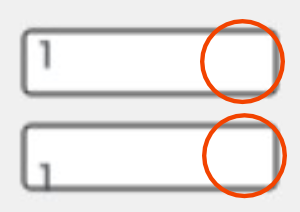
\includegraphics[scale=0.5]{bilder/NumericBoxPfeile.png}
    \caption{\texttt{NumericBox} mit fehlenden Buttons zum In- und Dekrementieren}
    \label{fig:numeric_box}
\end{figure}


In JADX werden darüber hinaus manche \gls{gui}-Elemente, wenn sie in einem zusätzlichen Fenster geöffnet werden, nicht angezeigt. Innerhalb der Box zur Eingabe numerischer Werte (\texttt{NumericBox}) werden die Buttons, durch welche der Wert in- oder dekrementiert werden kann, nicht angezeigt. Dies wird in Abb.~\ref{fig:numeric_box} dargestellt.
Weitere Unterschiede zwischen JADX und der Umsetzung des Mocks ergeben sich aus den Limitierungen von OrbTK in Verbindung mit der Umsetzungszeit. Wie in Abschnitt \ref{subsec:goal_mock} beschrieben ist, war es auch kein Ziel hinter der Entwicklung, JADX zu 100\% abzubilden. Viele Effekte, wie Schattierungen oder Verbindungslinien im Strukturbaum in der Hauptübersicht in Abb.~\ref{fig:mock_comparison}, sind so nicht in OrbTK vorhanden und nur mit unverhältnismäßigem Aufwand nachzubauen. Teilweise wurden auch \gls{gui}-Elemente implementiert, deren Design dem von JADX ähnlich ist, die jedoch keine Funktion haben. Ein Beispiel hierfür ist die Tab-Navigation über dem Editor. Die einzelnen Tabs sind nicht mit Daten hinterlegt, sodass bei einem Klick auf einen Tab nichts passiert. Da nur Abbilder der \gls{gui} verwendet werden und keine Aktionen ausgeführt werden, ist dies jedoch auch nicht notwendig. Features von JADX, wie die Speicherverbrauchsanzeige am unteren Fensterrand oder die kleinere Tabnavigation (\glqq Code\grqq\ und \glqq Smali\grqq ), wurden nicht umgesetzt.


% \begin{itemize}
%     \item Was wird für eine GUI benötigt?
%     \begin{itemize}
%         \item \textit{Welche Menüs?}
%         \item \textit{Welche Buttons? Wo platzieren?}
%         \item \textit{Styling?}
%     \end{itemize}
% \end{itemize}

\section{Implementierung der prozeduralen Generierung}
Die Ansichten der \gls{gui} müssen anschließend prozedural generiert werden. Da unstrukturierte, valide Ansichten zum Training der Autoencoder ausreichen, können zufällig neue Ansichten generiert werden. Wichtig hierbei ist, dass alle \gls{gui}-Elemente des Mocks, aber auch möglichst viele valide Konfigurationen und Kombinationen dieser Elemente, abgedeckt sind.
Im Proposal wurde die Frage aufgeworfen, ob die Generierung in Python oder Rust umgesetzt werden soll. Im ersten Fall müssten alle variablen Teile zur Verwendung durch Python freigegeben werden, womit die Schnittstelle zu Python komplexer werden würde. Dafür könnte der Quelltext, der die Generierung betrifft, in Python geschrieben werden, womit dieser Quelltext, wie im Proposal argumentiert, wartbarer, lesbarer und zugänglicher werden könnte. Letztere Argumentation hat sich im Lauf der Entwicklung als falsch herausgestellt. Durch die Kapselung in einen separatem Generator ist dieser sowohl wartbar als auch von der \gls{gui} separiert. Die Bedenken bezüglich der Lesbarkeit haben sich nicht bestätigt.
Daher wurde der Generator in Rust implementiert.

Um möglichst viel Variabilität von JADX abzudecken, ist ein hoher Grad an Randomisierung nötig. Jede Ansicht der Anwendung, die aus dynamischem Inhalt besteht, soll mit randomisiert generiertem Inhalt gefüllt werden. Dies betrifft den Projektbaum, die Tab-Navigation, den Inhalt des Editors, die Eingabefelder, Dropdown-Menüs~und~\mbox{Checkboxen}.

\subsection{Generator}
\label{subsec:generator}
Um \gls{gui}-Daten zu generieren, müssen sowohl der Inhalt als auch die Struktur erstellt werden. Die Struktur des Mocks bezeichnet dabei die geöffneten Fenster, die geöffneten Menüs und die Größe der Fenster. Die generierten Strukturelemente und deren Wahrscheinlichkeiten werden in Tab.~\ref{tab:window_probabilities} dargestellt. Die Wahrscheinlichkeit, dass ein zusätzliches Fenster angezeigt wird, beträgt $50\%$. Unter der Bedingung, dass \emph{kein} zusätzliches Fenster angezeigt wird, wird wiederum mit 50-prozentiger Wahrscheinlichkeit ein Menü angezeigt. Falls ein zusätzliches Fenster angezeigt wird, können gleichzeitig keine Menüs existieren. Die Gesamtwahrscheinlichkeit, ob ein solches Menü angezeigt wird, beträgt demnach $\frac{1}{4}$. Falls die Entscheidung, ob ein Menü bzw. Fenster  angezeigt wird, positiv ausfällt, wird die Entscheidung, welches Menü bzw. Fenster angezeigt wird, randomisiert anhand einer Gleichverteilung getroffen.

Der gesamte variable Inhalt des Mocks wird zufällig generiert. Dies bedeutet, dass alle Eingabefelder, Dropdown-Menüs und Checkboxen zufällig befüllt werden. Die möglichen Werte für die einzelnen Variationspunkte werden in Tab.~\ref{tab:variation_fields} beschrieben. In Tab.~\ref{tab:variation_components} werden weitere Komponenten beschrieben, deren Struktur generiert wird, die jedoch auch aus mehreren randomisiert generierten Bausteinen bestehen.

Die Wahrscheinlichkeiten wurden so gewählt, dass Ansichten mit einer höheren Komplexität häufiger gezeigt werden, als Ansichten mit einer geringeren Komplexität. Ein Menü mit einigen statischen Icons und statischem Text ist dabei wesentlich weniger komplex, als ein größeres Fenster mit entsprechend mehr und vor allem dynamisch generiertem Inhalt. Fenster wurden deshalb gegenüber Menüs im Generator stärker gewichtet ($p_{fenster}=\frac{1}{12}$ gegenüber $p_{menu}=\frac{1}{20}$). Die Menüs sowie die Fenster untereinander werden gleich häufig angezeigt, um ein gleichmäßiges Lernen der Elemente zu gewährleisten.

\subsection{Anmerkung}
An dieser Stelle ist es wichtig zu erwähnen, dass sich die Wahrscheinlichkeitsverteilung \emph{nicht} an der Wahrscheinlichkeitsverteilung bei einer realistischen Nutzung orientiert. Das Ziel des Generators ist es, das Training zu optimieren, und nicht, eine realitätsnahe Wahrscheinlichkeitsverteilung abzubilden. Ein häufiges Problem bei maschinellem Lernen ist, dass Randfälle in den Trainingsdaten unterrepräsentiert sind, wie etwa im Bereich des autonomen Fahrens~\cite{karunakaranEfficientStatisticalValidation2020}. Ein Vorteil des Ansatzes dieser Masterarbeit ist es, Randfälle beliebig und einfach stärker gewichten zu können. Falls notwendig kann diese Gewichtung auch nachträglich durch Neuerstellung des Datensatzes verändert werden.

% \newpage

\begin{figure}[p]
    \centering
    \renewcommand*{\arraystretch}{1.5}
    \begin{minipage}{\textwidth}
    \captionof{table}{Strukturelemente mit dazugehöriger Anzeigewahrscheinlichkeit}
    \label{tab:window_probabilities}
    \smallskip
    \begin{tabularx}{\textwidth}{ lX }
        \toprule
        Strukturelement & Anzeigewahrscheinlichkeit \\
        \hline
        kein zusätzliches Fenster & $P(X=kein Fenster) = 0,5$ \\
        Einstellungsfenster & $P(X=Einstellungen) = \frac{1}{12}$\\
        Textsuchfenster & $P(X=Textsuche) = \frac{1}{12}$ \\
        Klassensuchfenster & $P(X=Klassensuche) = \frac{1}{12}$ \\
        Suchfenster für Suche nach Benutzung & $P(X=Benutzungssuche) = \frac{1}{12}$ \\
        Fenster zur Umbenennung & $P(X=Umbenennung) = \frac{1}{12}$\\
        \glqq Über\grqq -Fenster & $P(X=\ddot{U}ber) = \frac{1}{12}$\\
        Kein Menü & $P(Y=keinMen\ddot{u})=0,25$, $P(keinFenster | Y=keinMen\ddot{u}) = 0,5$\footnote{$P(\neg keinFenster | Y=keinMen\ddot{u}) = 1 $} \\
        File-Menü & $P(Y=FileMen\ddot{u})=0,05$, $P(keinFenster | Y=FileMen\ddot{u}) = 0,1$\footnote{ $P(\neg keinFenster | Y=FileMen\ddot{u}) = P(\neg keinFenster | Y=ViewMen\ddot{u}) = \\ P(\neg keinFenster | Y=NavigationMen\ddot{u}) = P(\neg keinFenster | Y=ToolsMen\ddot{u}) = \\ P(\neg keinFenster | Y=HelpMen\ddot{u}) = 0 $\label{fn:tab:negate_prop}} \\
        View-Menü & $P(Y=ViewMen\ddot{u})=0,05$, $P(keinFenster | Y=ViewMen\ddot{u}) = 0,1$\footref{fn:tab:negate_prop} \\
        Navigation-Menü & $P(Y=NavigationMen\ddot{u})=0,05$, $P(keinFenster | Y=NavigationMen\ddot{u}) = 0.1$\footref{fn:tab:negate_prop} \\
        Tools-Menü & $P(Y=ToolsMen\ddot{u})=0,05$, $P(keinFenster | Y=ToolsMen\ddot{u}) = 0,1$\footref{fn:tab:negate_prop}\\
        Help-Menü & $P(Y=HelpMen\ddot{u})=0,05$, $P(keinFenster | Y=HelpMen\ddot{u}) = 0,1$\footref{fn:tab:negate_prop}\\
        \bottomrule
    \end{tabularx}
\end{minipage}
\end{figure}

%     \footnotetext[20]{ $P(\neg keinFenster | Y=FileMen\ddot{u}) = P(\neg keinFenster | Y=ViewMen\ddot{u}) = \\ P(\neg keinFenster | Y=NavigationMen\ddot{u}) = P(\neg keinFenster | Y=ToolsMen\ddot{u}) = \\ P(\neg keinFenster | Y=HelpMen\ddot{u}) = 0 $\label{fn:tab:negate_dprop}}


% \end{figure}

\begin{table}[p]
    \centering
    \caption{\glsxtrshort{gui}-Elemente mit generiertem Inhalt}
    \label{tab:variation_fields}
    \smallskip

\begin{tabularx}{\textwidth}{ XXX }
    \toprule
    Variationspunkt & Art der Befüllung & Inhaltsart \\
    \hline
    Checkbox & Zufällige Markierung & Ja/Nein \\
    Dropdown-Menü & Zufällige Auswahl & Statische Elemente \\
    Numerisches Feld & Zufällige Zahl & Realistischer Zahlenbereich (Bsp: 1..100) \\
    Text(-feld) & Zufälliger Text & Alphanumerischer Text mit Länge in bestimmtem Bereich \\
    Icon & Zufälliges Icon & Icons aus JADX (je nach Kontext nur Icons für Dateien oder Entitäten) \\
    \bottomrule
\end{tabularx}


\end{table}

\begin{table}[p]
    \centering
    \caption{JADX-Komponenten mit generierter Struktur und Inhalt}
    \label{tab:variation_components}
    \smallskip

\begin{tabularx}{\textwidth}{ XXX }
    \toprule
    Variationspunkt & Elemente & Art der Befüllung  \\
    \hline
    Tab-Navigation & Tabs bestehend aus Icon und Text & 1..10 Tabs \\
    Projektbaum & Einträge aus Icon und Text sowie Kindelementen & Baumstruktur: Jedes Element hat bis zu 10 Kindelemente, max. 100 Elemente \\
    Suchergebnisse & Einträge aus Icon sowie 2 Texten (In JADX Name der Entität und ein Code-Ausschnitt ) & Max. 20 Einträge (zeilenweise) \\

    \bottomrule
\end{tabularx}
\end{table}

% \begin{itemize}
%     \item Was ist das?
%     \begin{itemize}
%         \item Generierung der GUI über Parameter und Zufall
%         \item Implementierung in Python oder Rust?
%     \end{itemize}
%     \item Warum prozedural Generieren?
%     \item Was ist dabei wichtig?
% \end{itemize}
\section{Implementierung von Python-Bindings}
Im Proposal zu dieser Masterarbeit wurde vorgeschlagen Bindings zu schreiben, um eine Verwendung des Generators in Python zu ermöglichen.
Python-Bindings definieren die Schnittstelle, um Bibliotheken anderer Programmiersprachen in Python aufzurufen. Diese Technik wird häufig genutzt um die Geschwindigkeitsvorteile von in C, C++ oder Rust entwickelten Bibliotheken auch in Python zu nutzen.

Ursprünglich war es vorgesehen, Python-Bindings zu entwickeln, um den Generator innerhalb des PyTorch-Quelltexts zu starten. Im Zug des Entwicklungsprozesses traten jedoch Probleme mit Speicherlecks durch OrbTK bei der wiederholten Generierung von Bildern auf. Daher traf ich die Entscheidung, auf die Entwicklung von Python-Bindings zu verzichten und den Generator so umzubauen, dass er nur ein einziges Bild generiert. Ein Bash-Skript startet den Generator dann so oft, bis der Datensatz fertiggestellt ist. Der Generator wird so jedes Mal in einem neuen Prozess gestartet, wodurch keine Speicherlecks und Probleme mit der \gls{cpu}-Auslastung auftreten können. In der Praxis führt dies nicht zu Einschränkungen, da der Datensatz in der Regel nur ein Mal erstellt wird und später nur noch verwendet wird. Es kommt somit nicht zu einem nennenswertem Mehraufwand bei der Entwicklung der Autoencoder.

% Aktuell ist der Generator so aufgebaut, dass für jedes Bild eine neue Instanz von OrbTK in einem eigenen Thread gestartet wird, von welcher ein Screenshot erstellt wird. Für einen Datensatz von 1000 Bildern werden daher 1000 Instanzen geöffnet und geschlossen. Das Schließen der Instanzen scheint jedoch zum aktuellen Zeitpunkt nicht fehlerfrei zu funktionieren und resultiert in einem Speicherleck. Die \gls{cpu}-Auslastung steigt ebenso immer weiter an, bis sie 100\% erreicht und die Generierung der Bilder immer langsamer funktioniert. Die einzige Lösung für dieses Problem ist es, jeweils einen eigenen Prozess pro OrbTK-Instanz zu starten.


% \begin{itemize}
%     \item Warum?
%     \item Was ist das?
%     \begin{itemize}
%         \item Rust Code der von Python (beispielsweise über Pip Package) aufgerufen werden kann
%         \item Deklarierte Schnittstelle
%     \end{itemize}
%     \item Wie funktioniert das?
%     \begin{itemize}
%         \item PyO3 (\url{https://pyo3.rs})
%         \item Siehe Beispiele
%     \end{itemize}
% \end{itemize}

\section{Fazit}
Das Ergebnis der Entwicklung des Mocks ist insgesamt zufriedenstellend. Die Abweichungen zwischen JADX und dem Mock sind bis auf wenige Features und den Betriebssystemfunktionalitäten gering. Inwiefern diese Abweichungen für die Ergebnisse eine Role spielen wird in Kapitel~\ref{cha:autoencoder} besprochen.
Die Bewertung, ob solche Mocks in Zukunft eingesetzt werden sollen, fällt jedoch negativ aus. OrbTK bereitet insgesamt durch ein schlechtes Layout-System, Speicherlecks, aktuell keiner Offscreen-Rendering-Unterstützung und andere Bugs zu viele Probleme. Es ist nur mit Aufwand möglich, einen solchen Mock zu erstellen, der dann auch produktiv eingesetzt werden kann. Alle weiteren untersuchten Frameworks sind ebenfalls noch in einem frühen Stadium und benötigen oft eine \gls{gpu}. Inwiefern letztere durch einen Software-Renderer ersetzt werden kann, ist zum jetzigen Stand zwar unklar, wäre jedoch auch nicht mehr als ein Workaround und damit prinzipiell nicht optimal.